\documentclass[12pt,a4paper]{report}

\usepackage[T1]{fontenc}
\usepackage[utf8]{inputenc}
\usepackage{lmodern}
\usepackage{microtype}
\usepackage{geometry}
\geometry{margin=2.5cm}
\usepackage{setspace}
\onehalfspacing
\usepackage{graphicx}
\usepackage{booktabs}
\usepackage{amsmath,amssymb}
\usepackage{hyperref}
\hypersetup{colorlinks=true,linkcolor=blue,urlcolor=blue,citecolor=blue}
\usepackage[numbers,sort&compress]{natbib}

\graphicspath{{figures/}}

\title{\textbf{CALM: Continual Adaptive Learning Model with Self-Aware Readiness Agent}\\[0.5em]
\large for Reliable Few-Shot Vision Systems}
\author{%
\textbf{Adib Ar Rahman Khan\hspace{2em}ID : 2212708042\\ & Saumik Saha Kabbya\hspace{2em}ID : 2211204042}\\ %
}
\date{%
\textbf{Directed Research --- Fall,2025}\\[1em]
Faculty Advisor: \\ \textbf{Muhammad Shafayat Oshman} \\ Lecturer \\ ECE Department%
}

\begin{document}

\makeatletter
\begin{titlepage}
\begin{center}
\vspace*{-8mm}

\includegraphics[width=0.28\textwidth]{nsu}\\[14pt]

{\Large\textbf{Department of Electrical and Computer Engineering}\par}
\vspace{10pt}
{\Large\textbf{North South University}\par}
\vspace{36pt}

{\LARGE\@title\par}\vspace{2.2em}
{\large\@author\par}\vspace{2em}
\@date\par
\end{center}

\vfill
\vspace*{12mm}
\end{titlepage}
\makeatother

% --- Front matter (departmental convention) ---
\clearpage

\chapter*{Letter of Transmittal}
\addcontentsline{toc}{chapter}{Letter of Transmittal}

\begin{flushleft}
May 2026 \\
\vspace{0.5cm}
To \\
\textbf{Dr. Mohammad Abdul Matin} \\
Chairman, Department of Electrical and Computer Engineering \\
North South University, Dhaka-1229, Bangladesh \\

\vspace{0.5cm}
\textbf{Subject: Submission of Directed Research Report on ``CALM: Continual Adaptive Learning Model with Self-Aware Readiness Agent for Reliable Few-Shot Vision Systems''.}

\vspace{0.5cm}
Dear Sir,

With respect, we submit our directed research report on \textbf{``CALM: Continual Adaptive Learning Model with Self-Aware Readiness Agent for Reliable Few-Shot Vision Systems''}, prepared under course \textbf{CSE498R: Directed Research} in the Department of Electrical and Computer Engineering, North South University.

This document presents our investigation into continual and few-shot vision under frozen vision--language encoders, including CALM-v1 (prototypical classification with a calibrated readiness agent and human-in-the-loop memory updates) and CALM-v2 (multi-encoder fusion, disagreement-aware confidence, and hierarchical compressed memory). We summarize the methodology, experimental protocols on ImageNet-aligned benchmarks, results, and conclusions drawn from this work.

We have endeavored to present the work clearly and faithfully, and we trust that the report will meet the expectations of the course and the department.

\vspace{1cm}
Sincerely yours,

\vspace{1.5cm}
\begin{tabular}{cc}
\rule{6cm}{0.4pt} & \rule{6cm}{0.4pt} \\
\textbf{Adib Ar Rahman Khan} & \textbf{Saumik Saha Kabbya} \\
ID: 2212708042 & ID: 2211204042
\end{tabular}
\end{flushleft}

\clearpage

\chapter*{Approval}
\addcontentsline{toc}{chapter}{Approval}

The directed research report titled \textbf{``CALM: Continual Adaptive Learning Model with Self-Aware Readiness Agent for Reliable Few-Shot Vision Systems''} submitted by \textbf{Adib Ar Rahman Khan (2212708042)} and \textbf{Saumik Saha Kabbya (2211204042)} under the supervision of \textbf{Muhammad Shafayat Oshman}, Lecturer, Department of Electrical and Computer Engineering, North South University, has been accepted as satisfactory for the partial fulfillment of the requirements for the course \textbf{CSE498R: Directed Research} toward the degree of Bachelor of Science in Computer Science and Engineering.

\vspace{3cm}
\begin{center}
\begin{tabular}{cc}
\rule{6cm}{0.4pt} & \rule{6cm}{0.4pt} \\
\textbf{Muhammad Shafayat Oshman} & \textbf{Dr. Mohammad Abdul Matin} \\
Lecturer & Chairman \\
Department of ECE & Department of ECE \\
North South University & North South University
\end{tabular}
\end{center}

\clearpage

\chapter*{Declaration}
\addcontentsline{toc}{chapter}{Declaration}

This is to declare that this project/directed research is our original work. No part of this work has been submitted elsewhere partially or fully for the award of any other degree or diploma. All project related information will remain confidential and shall not be disclosed without the formal consent of the project supervisor. Relevant previous works presented in this report have been properly acknowledged and cited. The plagiarism policy, as stated by the supervisor, has been maintained.  

\vspace{3cm}
\begin{center}
\begin{tabular}{cc}
\rule{6cm}{0.4pt} & \rule{6cm}{0.4pt} \\
\textbf{Adib Ar Rahman Khan} & \textbf{Saumik Saha Kabbya} \\
ID: 2212708042 & ID: 2211204042
\end{tabular}
\end{center}

\clearpage

\chapter*{Acknowledgment}
\addcontentsline{toc}{chapter}{Acknowledgment}

We express our sincere gratitude to our faculty advisor, \textbf{Muhammad Shafayat Oshman}, Lecturer, Department of Electrical and Computer Engineering, North South University, for guidance, feedback, and support throughout this directed research. His direction on problem formulation, experimental design, and presentation of results has been essential to completing this work.

We thank the \textbf{Department of Electrical and Computer Engineering} at North South University for the academic environment and resources that made this project feasible.

We are also grateful to our families and peers for their encouragement during the course of this research.

\clearpage

\begin{abstract}
\noindent
Large-scale multimodal alignment has produced extraordinarily reusable visual encoders whose latent geometries already separate thousands of coarse-grained categories when paired with simple decision rules or textual prompts. Industrial adoption nevertheless struggles when labeled supervision trickles slowly, workloads evolve through many deployment cycles without permission to refactor backbone weights after certification, and product teams insist on interpretable escalation paths instead of brittle always-on autonomy. This report documents the \emph{Continual Adaptive Learning Model} (CALM), instantiated in two engineering variants that mirror our companion technical manuscript: \textbf{CALM-v1} couples a frozen vision--language trunk with episodic memory, prototypical (centroid-based) scoring, and a temperature-calibrated \emph{readiness agent} that gates autonomous deployment against human-in-the-loop label acquisition; \textbf{CALM-v2} augments that stack with multi-encoder score fusion, disagreement-aware confidence summaries, and hierarchically compressed memory tiers aimed at long-horizon operation. We summarize the formal objectives and notation, reproduce ImageNet-aligned episodic and continual protocols (five-way five-shot episodic learning with six hundred episodes; ten-task continual learning with constrained rehearsal), and interpret measured trade-offs between episodic accuracy, average continual accuracy, and backward transfer. The narrative emphasizes that non-parametric adaptation under frozen representations is a viable deployment posture when reliability constraints dominate, while also underscoring open systems questions---especially geometric consistency across fused embedding spaces---that connect this work to broader debates on uncertainty, oversight, and scalable memory in foundation-model pipelines.
\end{abstract}

\clearpage
\tableofcontents
\clearpage
\listoffigures
\listoftables
\clearpage

\chapter{Introduction}

\section{Background and Motivation}
Computer vision workloads increasingly begin with heavyweight vision-language encoders pretrained through contrastive captioning pipelines~\cite{r1}. These models export fixed feature maps suitable for zero-shot transfer when natural-language prototypes exist, yet many enterprise monitoring scenarios mandate rapid specialization from only a handful of exemplars---precisely the operating point studied by episodic centroid learners~\cite{r3} and resurrected residual cache adaptations~\cite{r4}. Calibration research shows that softmax magnitudes seldom equal long-run hit rates unless temperature corrections or held-out regressions constrain them~\cite{r5}; deployment teams therefore need explicit abstention thresholds rather than naïvely trusting raw logits.

Continual learning literature documents complementary axes: quadratic regularizers such as elastic weight consolidation discourage drift in parameter space~\cite{r6}, rehearsal variants such as iCaRL replay exemplars alongside evolving linear heads~\cite{r7}, latent-replay formulations demonstrate that foundation encoders amortize rehearsal when representations stay frozen~\cite{r9}, while prompt-centric continual transformers rewrite internal conditioning tokens rather than rewriting convolutional weights outright~\cite{r8,r17}. These references collectively stress that multitask leaderboard scores often track methods that intervene inside backbone pathways, motivating our choice to carve out a transparent alternative when frozen-trunk contracts preclude risky fine tuning~\cite{r16}.

Uncertainty quantification and human oversight further frame deployment. Conformal ideas encourage reporting coverage-qualified sets instead of brittle scalars alone~\cite{r10}; multimodal extensions extrapolate analogous logic to heterogeneous encoders~\cite{r21}; pragmatic human-feedback frameworks articulate how sparing expert labels tame unstable LVLM cascades~\cite{r24}; and calibrated HRI studies remind us that robotic perception stacks must pair confidence telemetry with conservative actuation~\cite{r25}. These threads justify why CALM treats memory growth, calibration, and governance as first-class design variables rather than afterthought post-processing.

The North South University Directed Research summarized here instantiates CALM atop open CLIP artifacts~\cite{r1} and ImageNet-1k curricula~\cite{r2} so benchmarking scripts remain comparable across published baselines spanning prototypical episodic nets~\cite{r3}, training-free VL adapters~\cite{r4}, and parameter-efficient multimodal adaptations~\cite{r14,r15}. We emphasize transparent logging of centroid statistics, cosine temperatures, disagreement spreads, compression losses, and human-review queues so auditors can correlate metric shifts with design decisions---an ethos aligned with continual-learning evaluation hygiene and metric discipline~\cite{r19}.

\section{Purpose and Goal of the Project}
The central purpose of this Directed Research effort is fourfold:
\begin{enumerate}\setlength\itemsep{0.35em}
  \item Unify frozen multimodal encoders, episodic centroids, and readiness-oriented confidence flows into one reproducible toolkit;
  \item Document how hierarchical compression ideas imported from frontier-scale multimodal stacks~\cite{r31,r32} interplay with quantized replay buffers constrained to five-shot memories per category;
  \item Compare CALM variants against heterogeneous literature excerpts under deliberately matched protocol generators to avoid exaggerated gains;
  \item Translate empirical regressions affecting the dual-encoder instantiation into pragmatic guidance about metric-space alignment and separation of roles between classifier logits versus abstention probes~\cite{r5,r10}.
\end{enumerate}
Goal three explicitly targets engineering repeatability: the same codebase seeds episodic curricula, multitask curricula, readiness threshold sweeps, and audit logs so supervising faculty may trace every figure in this dossier back to deterministic manifests.

\section{Organization of the Report}
Chapter~\ref{ch:lit} surveys vision--language foundations and benchmarks~\cite{r1,r2,r27}, meta-learning and training-free adapters~\cite{r3,r4}, parameter-efficient multimodal tuning~\cite{r11,r12,r13,r14,r15,r16}, continual learning and prompting~\cite{r6,r7,r8,r9,r17,r18,r19,r20}, reliability and human oversight~\cite{r5,r10,r21,r22,r23,r24,r25,r26}, smaller-scale recognition corpora~\cite{r28,r29,r30}, and hierarchical multimodal memory at scale~\cite{r31,r32}. Chapter~\ref{ch:meth} details requirements, methodology, tooling, figures, and implementation. Chapter~\ref{ch:res} lays out investigation objectives, episodic and continual protocols, reproducibility practices, tabulated results~\cite{r2,r3,r4}, multi-level analysis (v1 vs.\ v2, temperature, fusion), discussion of threats to validity~\cite{r19}, and deployment-facing interpretation~\cite{r23,r24,r25}. Chapter~\ref{ch:con} states limitations---partial readiness analytics for CALM-extensions, unfinished single-backbone ablations, and reliance on predominantly natural photographic corpora akin to foundational recognition surveys~\cite{r29,r30}---and charts future conformance studies~\cite{r10,r22}. The bibliography lists thirty-two numbered sources with authors spelled out in full (following the departmental specification).

\chapter{Research Literature Review}
\label{ch:lit}

This chapter positions CALM within a deliberately wide sweep of adjacent research. The breadth is purposeful: CALM intersects frozen foundation encoders~\cite{r1}, episodic inference~\cite{r3}, continual task streams~\cite{r7,r8}, calibrated deployment policies~\cite{r5,r10}, and memory-scaling motifs from frontier vision--language stacks~\cite{r31,r32}. We proceed from transferable representations toward adaptation strategies, continual-learning paradigms, reliability and governance, benchmarking assumptions, multimodal architectures, and finally the niche CALM occupies.

\section{Vision--language alignment, transfer, and survey perspectives}
Contrastive captioning pipelines such as CLIP~\cite{r1} map images and paired text into a shared embedding space, enabling zero-shot classifiers induced from natural-language prompts and serving as ubiquitous feature extractors for downstream vision~\cite{r27}. Architectural scale and curated web-scale pairing explain much of zero-shot breadth, yet transfer quality remains sensitive to domain shift~\cite{r27}: off-the-shelf ImageNet-aligned metrics~\cite{r2} summarize one convenient operating point rather than guaranteeing robustness across sensors, modalities, or long-tailed deployments. Survey literature~\cite{r27} therefore distinguishes \emph{what} pretrained geometry provides from \emph{how} responsibly to adapt---a distinction central to CALM, which freezes $\theta$ and treats adaptation as episodic reasoning on top of a fixed metric.

\section{Few-shot learning, meta-learning, and training-free adaptation}
Classical meta-learning aspired to learn update rules or initialization points that generalize across tasks; prototypical networks~\cite{r3} showed that simple class centroids in embedding space, combined with episodic training, already yield strong inductive bias for few-shot classification. In the CLIP era, analogous ``centroid'' stories reappear when supports are few and the backbone is frozen: rather than meta-training the encoder, one meta-trains \emph{only} the decision rule (or cache) on features. Tip-Adapter~\cite{r4} exemplifies \emph{training-free} residual adaptation---augmenting logits with a lightweight key--value cache over training-free CLIP embeddings---and reports competitive accuracy without trunk updates. CALM-v1 borrows the \emph{spirit} of prototype reasoning~\cite{r3} but routes adaptation through explicit episodic memory and human-in-the-loop refresh (Chapter~\ref{ch:meth}), whereas cache-style adapters~\cite{r4} typically assume batch or offline cache construction rather than a closed-loop operational contract.

\section{Parameter-efficient fine-tuning, adapters, and when to touch the trunk}
When organizations \emph{can} modify parameters, adapter insertions~\cite{r12}, prompt tuning~\cite{r11}, and low-rank updates such as LoRA~\cite{r13} reduce trainable mass relative to full fine tuning. Multimodal parameter-efficient recipes consolidate under adapter and VL-Adapter taxonomies~\cite{r14,r15}. Empirical ``how to train your CLIP'' guidance~\cite{r16} clarifies when modest in-domain fine tuning repays the cost of breaking immutability. CALM deliberately occupies the complementary regime: $\|\theta_{\text{adapted}}-\theta_{\text{original}}\|_2=0$ by design, deferring future hybrid studies (e.g., selective LoRA within certified subspaces~\cite{r13}) to follow-on work.

\section{Continual learning: consolidation, rehearsal, prompts, and foundation latents}
Catastrophic forgetting~\cite{r6} motivated regularization toward important weights, yet rehearsal often remains the practical workhorse when representational drift must be explicit~\cite{r7}. Prompt-based continual learners such as L2P~\cite{r17} and DualPrompt~\cite{r8} maintain task-aware conditioning in transformer blocks, frequently achieving high average accuracy on sequential benchmarks at the price of altering internal activations---a different contract than frozen-feature pipelines. Recent empirical studies~\cite{r9} argue that \emph{latent replay} (rehearsal in embedding space) can be effective when foundation representations are stable, anticipating CALM's philosophy of memory in $f_\theta(\cdot)$ space.

Surveys on continual learning for deep networks~\cite{r19} and for large language models~\cite{r18} stress evaluation hygiene: backward transfer, forward transfer, and protocol sensitivity matter as much as headline averages. Complementary lines on OOD-robust continual objectives~\cite{r20} remind us that sequential streams couple forgetting with distributional shift; CALM's readiness layer is conceptually adjacent to deferral under shift, even though our ImageNet-aligned experiments emphasize protocol comparability over exhaustive OOD sweeps.

\section{Calibration, conformal-style uncertainty, and multimodal reliability}
Modern classifiers are often miscalibrated out of the box~\cite{r5}; temperature scaling and related post-hoc adjustments align estimated confidences with empirical error rates on held-out data. Distribution-free tools such as conformal prediction~\cite{r10} provide coverage-style guarantees under exchangeability assumptions, motivating separation between \emph{classification} outputs and \emph{selective} deployment policies. Multimodal extensions~\cite{r21} begin to address ensembles of vision--language scores where geometry and score scales may disagree---precisely the tension that resurfaces when CALM-v2 fuses heterogeneous frozen encoders. Literature on LLM calibration~\cite{r26} reinforces that scalar confidence surfaces are brittle under prompt and domain perturbations.

Parallel threads on abstention-aware and out-of-distribution-aware large-model decision rules~\cite{r22}, hallucination characterization in large vision--language models~\cite{r23}, pragmatic human-feedback loops~\cite{r24}, and calibrated perception in robotics~\cite{r25} collectively argue that trustworthy deployment stacks require instrumentation beyond accuracy: escalation paths, abstention dashboards, and auditable rationales tied to thresholds. CALM's readiness agent~\cite{r5} is a deliberate, lightweight nod to that broader reliability agenda~\cite{r10,r24}.

\section{Benchmark ecology, domain breadth, and generalization claims}
Recognition benchmarks~\cite{r2,r28,r29,r30} differ in resolution, imbalance, semantics, and domain: ImageNet~\cite{r2} dominates vision leaderboards yet reflects natural photographs; legacy ``tiny''~\cite{r28} and STL-style~\cite{r29} splits probe low-resolution habits; Fashion-MNIST~\cite{r30} substitutes texture statistics for photographic scenes. Comparative claims must therefore caveat \emph{which} data manifold a method has been exercised on~\cite{r28,r29,r30}: CALM's directed research evaluation emphasizes ImageNet-structured episodic and continual partitions~\cite{r2} precisely for leaderboard alignment, without implying saturation on heterogeneous industrial domains~\cite{r27}.

\section{Scalable multimodal memory, mixture-of-experts, and compression}
Industrial vision--language systems increasingly discuss hierarchical memory, document-scale reasoning, and mixture-of-experts routing~\cite{r32}, sometimes alongside OCR-centric pipelines that ingest dense text~\cite{r31}. Architectural memoirs~\cite{r31,r32} justify tiered fidelity: recent context at full precision, summarized or compressed strata for archival traces, and disciplined routing rather than uniformly expanding parameter or token budgets. CALM-v2's hierarchical quantization heuristically mirrors that design ethos at laboratory scale without claiming production-scale provenance for our prototype.

\section{Synthesis: research gap and CALM positioning}
Individually, the cited threads are mature: transferable VL encoders~\cite{r1,r27}, meta-style few-shot summaries~\cite{r3}, cache adapters~\cite{r4}, PEFT catalogs~\cite{r12,r13,r14,r15}, continual prompting~\cite{r8,r17,r19}, calibration~\cite{r5,r26}, conformal viewpoints~\cite{r10,r21}, human-in-the-loop practice~\cite{r24}, hallucination-awareness~\cite{r23}, robotics calibration~\cite{r25}, latent replay~\cite{r9}, and multimodal scalability~\cite{r31,r32} each address important slices of the puzzle.

Relatively under-emphasized in prior work---as a single, logged engineering stack---are deployments that simultaneously (i)~forbid backbone mutation by policy while relying on frozen VL representations~\cite{r1}; (ii)~implement non-parametric prototype adaptation with episodic memory and closed-loop auditor updates~\cite{r3,r7,r24}; (iii)~bind autonomous operation to calibrated scalar readiness and tuned autonomy rates~\cite{r5,r10}; (iv)~experiment with disagreement across frozen encoders and lossy hierarchical memory~\cite{r21,r31,r32}; and (v)~report both few-shot episodic~\cite{r2,r3,r4} and multitask regressions~\cite{r7,r8} under transparent protocols~\cite{r19}. That lacuna motivates CALM as an integrative Directed Research artifact: broadly situated against VLMs and continual learning~\cite{r18,r27}, deliberately trunk-frozen by design~\cite{r1}, informed by literature on constrained CLIP adaptation~\cite{r16}, forthright about multitask compromises relative to prompt-tuned continual leaders~\cite{r8,r17}, and anchored in reproducible departmental reporting~\cite{r19} rather than leaderboard cherry-picking.

\chapter{Methodology}
\label{ch:meth}

The methodological exposition below follows the mathematical development of the CALM manuscript (anonymous NeurIPS-style submission), restated here in self-contained form for the Directed Research record. We first state the optimization constraints that motivate non-parametric adaptation, then derive CALM-v1 (single frozen encoder, flat episodic memory, prototypical classifier, readiness gating), and finally summarize CALM-v2 (multi-encoder fusion, disagreement statistics, hierarchical compressed memory). Each family of equations is accompanied by a concise interpretation of its symbols.

\section{Problem formulation}
We consider a pretrained vision--language model with image encoder $f_\theta : \mathcal{X} \to \mathbb{R}^d$, where $\mathcal{X}$ denotes the space of input images and $d$ the embedding dimension. Given a task $\mathcal{T} = \{(\mathbf{x}_i, y_i)\}_{i=1}^{n}$ with $K$ classes, the goal is to adapt predictions while keeping the backbone's semantic prior intact. Following the formalization in the paper, adaptation is required to satisfy three constraints:
\begin{align}
  &\text{(Efficiency)} && \mathcal{O}(\text{adaptation}) \ll \mathcal{O}(\text{fine-tuning}), \label{eq:efficiency}\\
  &\text{(Preservation)} && \|\theta_{\text{adapted}} - \theta_{\text{original}}\|_2 = 0, \label{eq:preservation}\\
  &\text{(Reliability)} && P(\text{error} \mid \text{deploy}) \le \epsilon. \label{eq:reliability}
\end{align}
Here $\theta$ indexes the \emph{frozen} trunk parameters; CALM satisfies~\eqref{eq:preservation} by construction (no gradient steps on $\theta$), addresses~\eqref{eq:efficiency} through memory-based rules instead of full fine tuning, and operationalizes~\eqref{eq:reliability} via the readiness agent and threshold calibration on validation episodes. The tolerance $\epsilon$ is set by the deployment context (risk budget).

\begin{table}[htbp]
  \centering
  \caption{Primary mathematical notation used throughout this report (consistent with the CALM paper).}
  \label{tab:notation}
  \begin{tabular}{@{}p{2.2cm}p{11.5cm}@{}}
    \toprule
    \textbf{Symbol} & \textbf{Meaning} \\
    \midrule
    $\mathbf{x}, \mathbf{e}$ & Input image and its $d$-dimensional embedding $\mathbf{e} = f_\theta(\mathbf{x})$. \\
    $\mathcal{M}$ & Episodic memory of tuples $(\mathbf{e}_i, y_i)$ (CALM-v1); tiered / multi-view extensions in v2. \\
    $S_k$ & Support set for class $k$ within $\mathcal{M}$. \\
    $\mathbf{c}_k$ & Class prototype (centroid) for label $k$. \\
    $\tau$, $T$ & Temperature in the classifier softmax ($\tau$) and in the calibrated readiness head ($T$); in general $T$ is tuned on validation data. \\
    $p(y{=}k\mid\mathbf{x})$ & Prototypical class posterior from cosine similarities. \\
    $q_x$ & Scalar confidence (maximum calibrated probability) driving the readiness decision. \\
    $\delta$, $\rho$ & Deployment threshold on $q_x$ and target autonomous deployment rate on validation data. \\
    $\mathcal{A}$ & Readiness map $\mathbb{R}^K \to \{0,1\}$ (request human review vs.\ deploy). \\
    $\mathcal{V}$, $v$ & Index set and index for frozen encoders in CALM-v2 (e.g.\ ViT-B/32 and ViT-B/16). \\
    $\mathbf{s}^{(v)}$, $\bar{\mathbf{s}}$ & Per-backbone similarity vectors and their nonnegative weighted fusion. \\
    $\sigma_x$ & Spread of per-backbone confidences (e.g.\ standard deviation across views), a disagreement signal. \\
    \bottomrule
  \end{tabular}
\end{table}

\section{CALM-v1: frozen encoder, memory, prototypes, and readiness}
\paragraph{Feature extraction.}
The trunk acts as a fixed feature map:
\begin{equation}
  \mathbf{e} = f_\theta(\mathbf{x}) \in \mathbb{R}^d,
\end{equation}
with the training-time constraint $\nabla_\theta \mathcal{L} = 0$ (no loss backpropagated into backbone weights during CALM adaptation).

\paragraph{Episodic memory and prototypical classification.}
Adaptation is mediated by an explicit memory
\begin{equation}
  \mathcal{M} = \{(\mathbf{e}_i, y_i)\}_{i=1}^{N},
\end{equation}
where each stored tuple pairs an embedding with its discrete label $y_i \in \{1,\ldots,K\}$. Class prototypes are centroid statistics over per-class supports $S_k = \{(\mathbf{e}_i,y_i)\in\mathcal{M} : y_i=k\}$:
\begin{equation}
  \mathbf{c}_k = \frac{1}{|S_k|} \sum_{(\mathbf{e}_i, y_i) \in S_k} \mathbf{e}_i.
  \label{eq:prototype}
\end{equation}
Query classification uses cosine similarity logits passed through a softmax with temperature $\tau$:
\begin{equation}
  p(y=k\mid\mathbf{x}) = \frac{\exp\bigl(\cos(\mathbf{e}_x, \mathbf{c}_k)/\tau\bigr)}{\sum_{j=1}^{K} \exp\bigl(\cos(\mathbf{e}_x, \mathbf{c}_j)/\tau\bigr)},
  \label{eq:classification}
\end{equation}
where $\mathbf{e}_x = f_\theta(\mathbf{x})$. This construction links CALM-v1 directly to prototypical inference~\cite{r3} while exploiting CLIP geometry~\cite{r1}.

\paragraph{Calibrated readiness and human-in-the-loop updates.}
The readiness agent compresses the vector of class scores into a scalar confidence and compares it to a policy threshold. Using temperature $T$ (possibly distinct from $\tau$) for calibration~\cite{r5},
\begin{equation}
  q_x = \max_k \frac{\exp\bigl(\cos(\mathbf{e}_x, \mathbf{c}_k)/T\bigr)}{\sum_{j=1}^{K} \exp\bigl(\cos(\mathbf{e}_x, \mathbf{c}_j)/T\bigr)}.
  \label{eq:calibration}
\end{equation}
The calibration temperature is chosen by minimizing negative log-likelihood on a held-out validation set:
\begin{equation}
  T^\ast = \arg\min_T \sum_{i=1}^{n_{\mathrm{val}}} -\log p\bigl(y_i \mid \mathbf{x}_i; T\bigr).
  \label{eq:temperature_opt}
\end{equation}
The binary deploy / request decision is
\begin{equation}
  \mathcal{A}(q_x) =
  \begin{cases}
    1 \;\text{(Deploy)} & \text{if } q_x \ge \delta,\\
    0 \;\text{(Request)} & \text{if } q_x < \delta,
  \end{cases}
  \label{eq:decision}
\end{equation}
with threshold $\delta$ tuned so that the empirical deployment rate on validation episodes matches a target $\rho$:
\begin{equation}
  \delta^\ast = \arg\min_{\delta} \Biggl| \frac{1}{n_{\mathrm{val}}} \sum_{i=1}^{n_{\mathrm{val}}} \mathcal{A}(q_i) - \rho \Biggr|.
  \label{eq:threshold_opt}
\end{equation}
When $\mathcal{A}(q_x)=0$, an expert supplies $y_{\mathrm{correct}}$ and memory expands without touching $\theta$:
\begin{equation}
  \mathcal{M} \leftarrow \mathcal{M} \cup \{(f_\theta(\mathbf{x}), y_{\mathrm{correct}})\},
  \label{eq:memory_update}
\end{equation}
which redefines affected prototypes via~\eqref{eq:prototype}. Thus adaptation is \emph{non-parametric} at the level of the backbone yet \emph{closed-loop} with respect to operational data.

\section{CALM-v2: multi-encoder fusion, disagreement, and hierarchical memory}
CALM-v2 preserves constraints~\eqref{eq:efficiency}--\eqref{eq:reliability} but revises how confidences are formed and how memory scales. Let $\mathcal{V}$ index a small set of frozen encoders $\{f_\theta^{(v)}\}_{v\in\mathcal{V}}$ (in our experiments, parallel CLIP scales such as ViT-B/32 and ViT-B/16~\cite{r1}). Each view maintains memory $\mathcal{M}^{(v)}=\{(\mathbf{e}^{(v)}_i,y_i)\}$ with $\mathbf{e}^{(v)}_i=f_\theta^{(v)}(\mathbf{x}_i)$ and prototypes $\mathbf{c}^{(v)}_k$ analogously to~\eqref{eq:prototype}. Per-backbone similarity vectors $\mathbf{s}^{(v)}\in\mathbb{R}^K$ collect logits $s^{(v)}_k = \cos(\mathbf{e}^{(v)}_x,\mathbf{c}^{(v)}_k)$ (or a fixed rescaling thereof), paralleling the scores underlying~\eqref{eq:classification}.

\paragraph{Fusion and disagreement-aware readiness.}
Nonnegative weights $\{w_v\}$ yield a fused score vector
\begin{equation}
  \bar{\mathbf{s}} = \frac{1}{\sum_{v\in\mathcal{V}} w_v} \sum_{v\in\mathcal{V}} w_v\, \mathbf{s}^{(v)},
\end{equation}
\begin{equation}
  \bar{p}_k = \frac{\exp(\bar{s}_k / T)}{\sum_{j=1}^{K} \exp(\bar{s}_j / T)}.
\end{equation}
The scalar $\max_k \bar{p}_k$ generalizes the v1 confidence $q_x$ in~\eqref{eq:calibration}. Disagreement across views is summarized separately---for example, with per-view maxima $q_x^{(v)} = \max_k p_k^{(v)}$ and spread $\sigma_x = \mathrm{std}_v(q_x^{(v)})$---so that readiness policies may map $(\max_k\bar{p}_k, \sigma_x)$ to deploy, defer, or request feedback, extending the binary rule~\eqref{eq:decision} in the spirit of reliability-aware multimodal systems~\cite{r10,r21}.

\paragraph{Hierarchical compression.}
Memory is partitioned into \emph{recent} (full precision), \emph{medium} (e.g.\ $512\!\to\!256$ bottleneck codes), and \emph{old} (stronger compression, e.g.\ $512\!\to\!128$, with optional subsampling) tiers~\cite{r31,r32}. When recomputing $\mathbf{c}_k$, compressed codes are decoded into the active backbone space before averaging; tier weights can down-rank highly lossy contributions. Compression modules are trained to reconstruct embeddings, keeping inference-time decompression lightweight.

\paragraph{Single-backbone ablation (conceptual).}
To separate representation inconsistency from memory design, the paper prescribes a variant that retains hierarchical memory but scores queries in a \emph{single} encoder space (typically ViT-B/32), restoring the metric coherence of v1 while preserving v2 memory mechanics.

Figures~\ref{fig:calm1}--\ref{fig:calm2} reproduce the pipeline diagrams from the submission PDF and should be read alongside the equations above.

\begin{figure}[htbp]
  \centering
  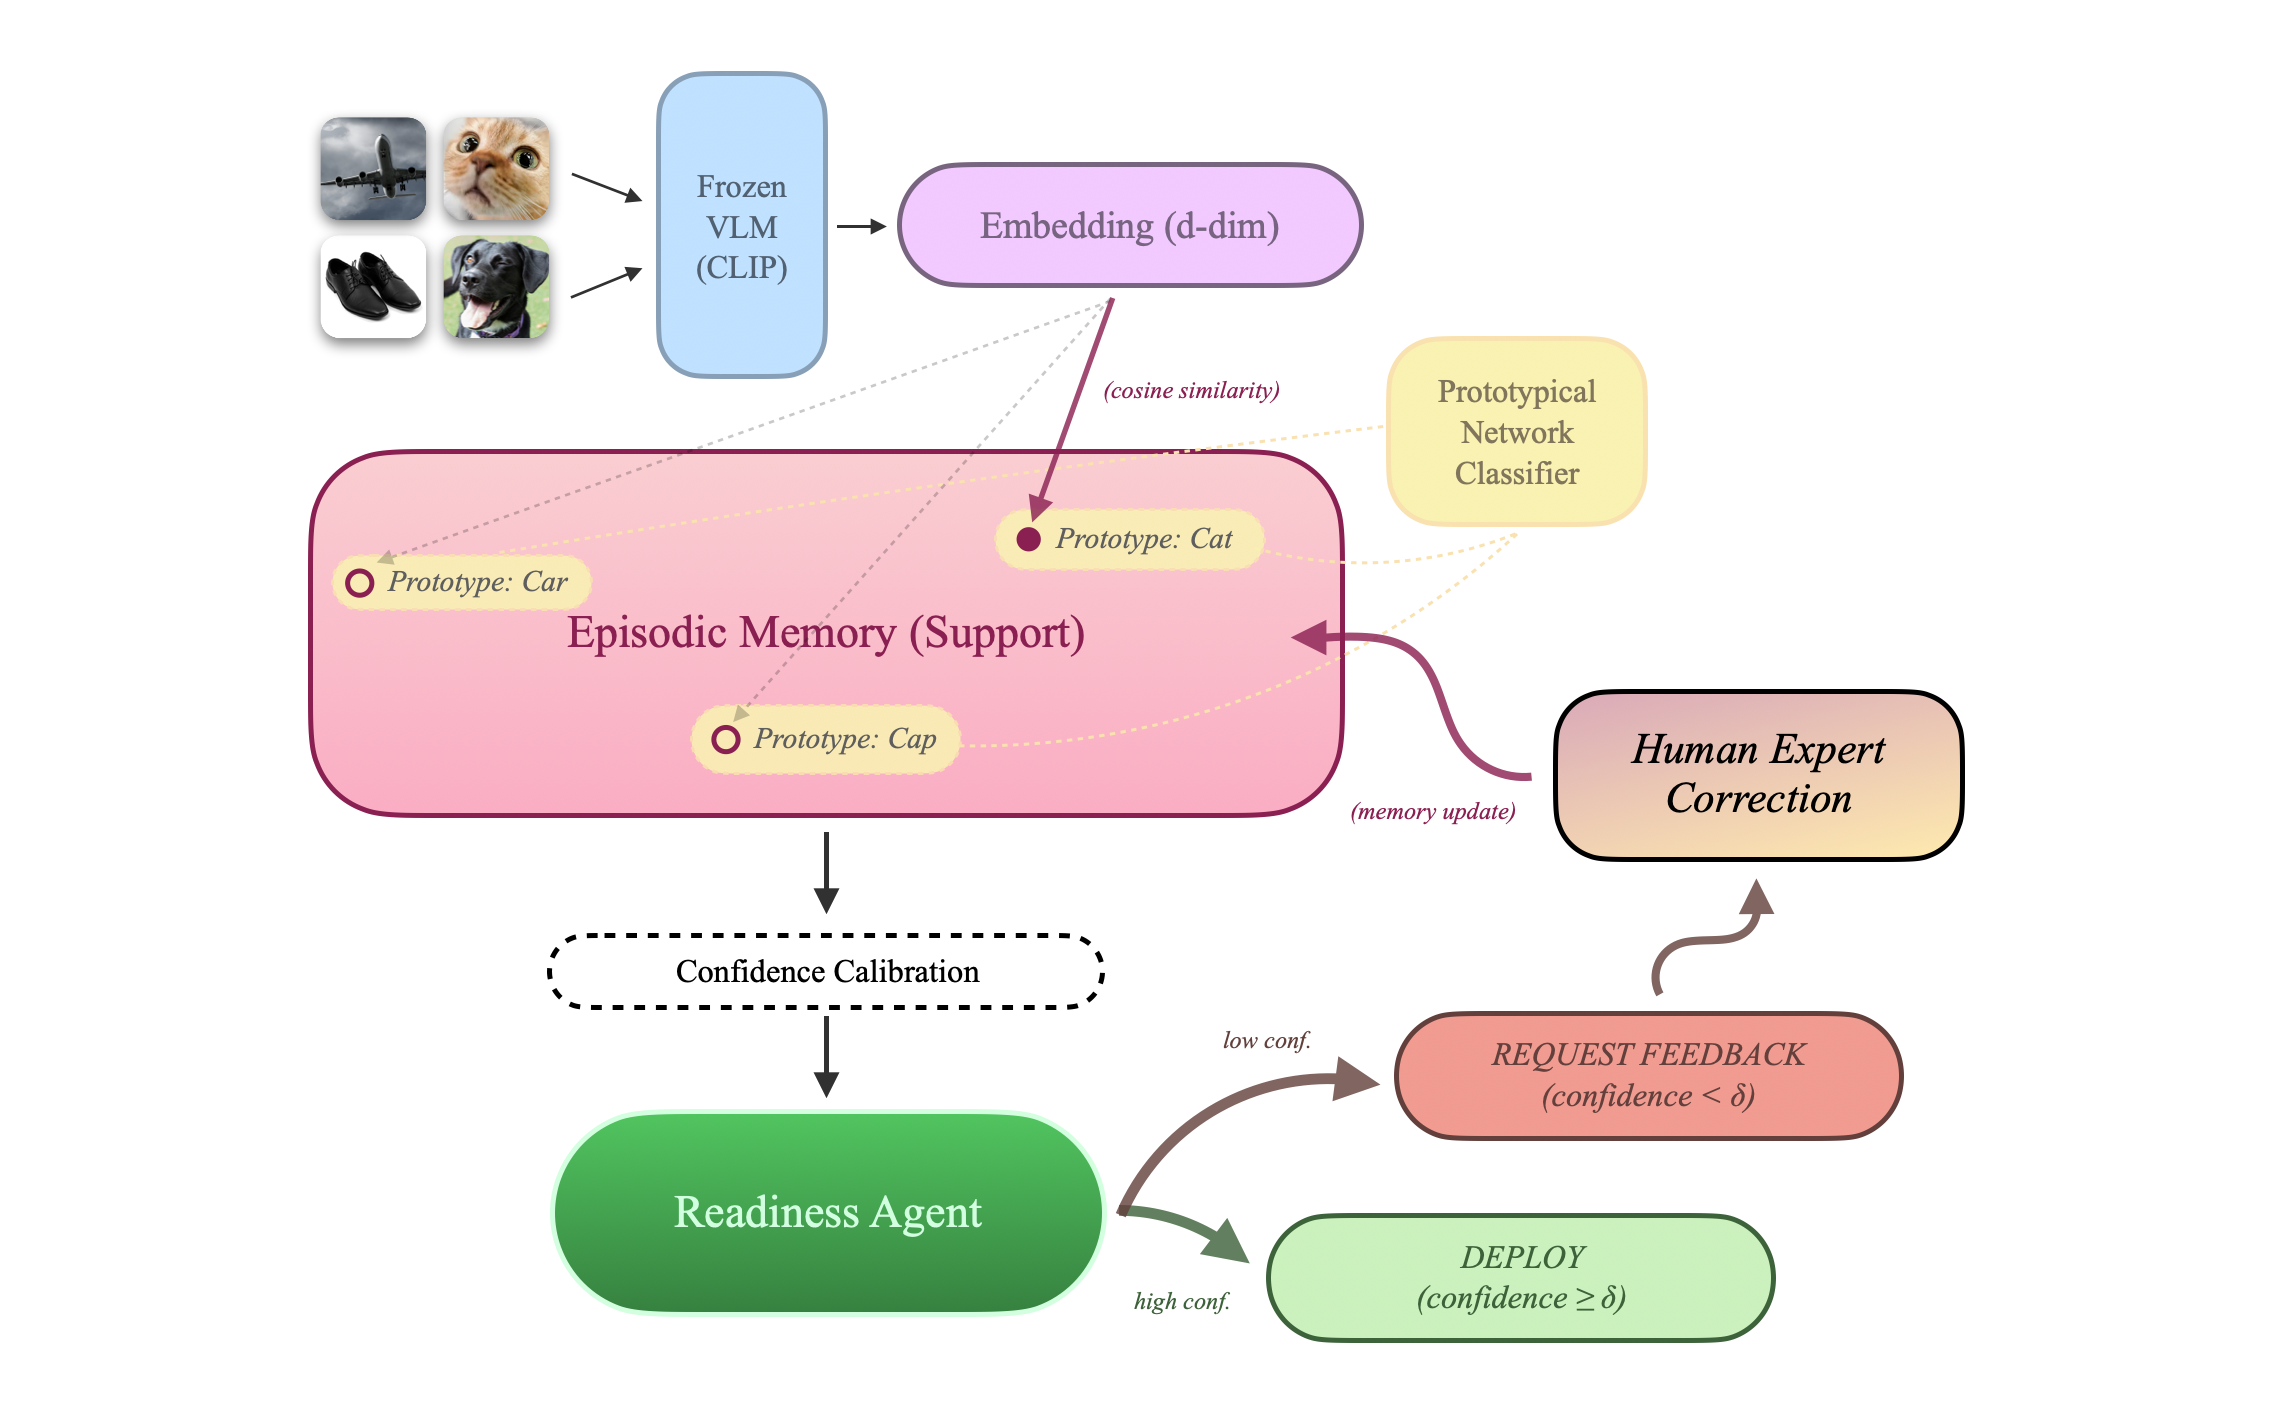
\includegraphics[width=0.95\textwidth]{extract_p5_xref146.png}
  \caption{CALM-v1 architecture: frozen CLIP encoder, episodic centroid classifier, calibrated readiness agent, and human-in-the-loop memory refresh.}
  \label{fig:calm1}
\end{figure}

\begin{figure}[htbp]
  \centering
  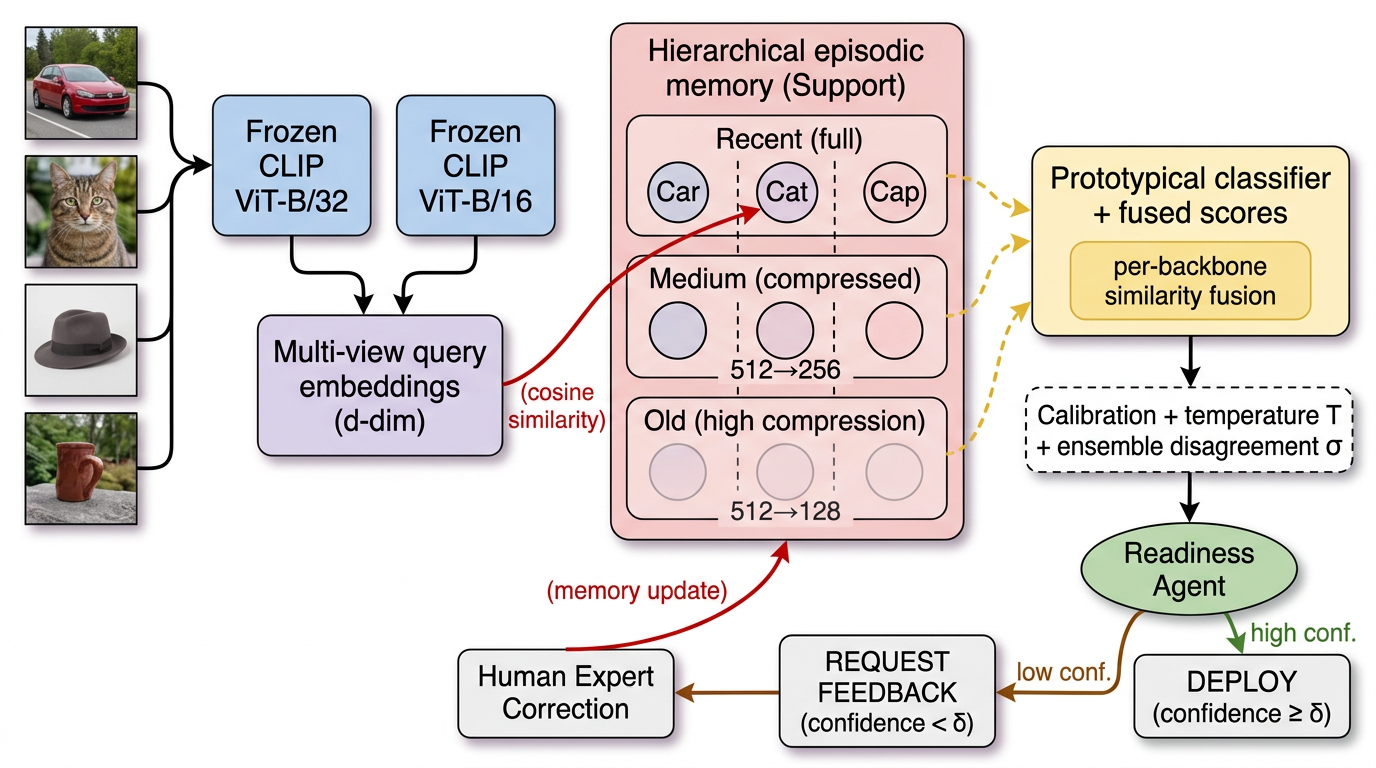
\includegraphics[width=0.95\textwidth]{extract_p6_xref191.png}
  \caption{CALM-extension schematic: dual CLIP-scale encoders, fused similarities, hierarchical memory tiers with compression, disagreement-aware readiness policy.}
  \label{fig:calm2}
\end{figure}

\section{Hardware and Software Components}
Hardware encompassed departmental GPU workstations with sufficient VRAM for batch embedding extraction without retraining gigantic transformers overnight. Primary software leveraged Python notebooks and reproducible launcher scripts, PyTorch interoperability with CLIP checkpoints, torchvision-style ImageNet indexers referencing the original CVPR database release~\cite{r2}, and experiment harnesses seeded for 600 episodic repetitions coupled to ten multitask phases mirroring benchmarking norms~\cite{r7,r8}. Supporting corpus snapshots~\cite{r28,r29,r30} contextualize risks when extrapolating beyond large-scale photographic domains.

\begin{table}[htbp]
  \centering
  \caption{Summary of principal software, checkpoint families, and dataset utilities.}
  \label{tab:tools}
  \begin{tabular}{p{3.6cm}p{4.2cm}p{3.2cm}p{3.2cm}}
    \toprule
    Tool & Functions & Comparable alternatives & Rationale \\
    \midrule
    Python stack (conda/venv) & Orchestration, sampling, reproducible logging. & Julia / R / MATLAB. & Ecosystem breadth for multimodal tooling. \\
    PyTorch-compatible CLIP (ViT-B/32 and ViT-B/16) & Immutable encoders, cosine-normalized embeddings. & Other foundation checkpoints. & Aligns with public VL baselines~\cite{r1}. \\
    ImageNet-1k partitioning utilities & Episodic and multitask curricula. & Other benchmarks. & Community comparability~\cite{r2}. \\
    \bottomrule
  \end{tabular}
\end{table}

\section{Hardware and/or Software Implementation}
Implementation milestones included hashing dataset manifests, versioning checkpoint checksums~\cite{r1}, deterministic episode RNG streams, centroid refresh hooks whenever human auditors append labeled tuples~\cite{r24}, dual-encoder cosine fusion logging with temperature grids~\cite{r5}, and tiered quantization pipelines validating reconstruction error before bits drop~\cite{r31,r32}. Continuous integration scripts bundle environment pins so downstream readers may rerun experiments without drifting dependencies.

\chapter{Investigation, Experiment, Results, Analysis, and Discussion}
\label{ch:res}

\section{Investigation objectives and empirical questions}
The empirical program behind this Directed Research pursued four intertwined questions anchored in~\eqref{eq:efficiency}--\eqref{eq:reliability}. First, can \emph{memory-centric} centroid adaptation over a frozen CLIP trunk~\cite{r1} match or exceed canonical training-free adapter baselines~\cite{r4} on standard ImageNet-derived episodic evaluation~\cite{r2,r3}? Second, under the same corpus, does that design remain workable when streams are elongated into multitask curricula with rehearsal budgets~\cite{r7,r9,r19}? Third, does extending confidence signals (ensemble fusion $\bar{\mathbf{s}}$) and compressing episodic strata~\cite{r31,r32} preserve few-shot competitiveness while materially changing continual aggregates? Fourth, how sensitive are observable metrics to calibrated temperature~\cite{r5} and fusion choices when multiple frozen encoders contribute scores~\cite{r21}? The sections below articulate how protocols, logging, tables, and discussion map each question onto measurable outcomes rather than speculative claims~\cite{r19}.

\section{Experimental protocols, metrics, and baseline heterogeneity}

\subsection*{Episodic few-shot classification}
All CALM variants follow the benchmarking protocol articulated in our companion CALM manuscript (anonymous NeurIPS-style submission), instantiated on ImageNet-1k~\cite{r2}. \textbf{Episodic classification} constructs many independent \emph{episodes}: in each episode, five classes $\mathcal{C}\subset \{1,\ldots,1000\}$ are sampled, five labeled supports are drawn uniformly per class, and fifteen queries are evaluated per class. We average accuracy over six hundred sampled episodes following standard episodic few-shot practice~\cite{r3}. This protocol foregrounds adaptation from sparse labels while keeping CLIP~\cite{r1} fixed in CALM---analogous in spirit to meta-evaluations of centroid rules~\cite{r3} except that embeddings are pretrained rather than co-trained episodically inside the episodic learner.

\textbf{Uncertainty reporting}: CALM-v1 is reported as a point estimate consistent with deterministic prototype refresh under fixed seeds; CALM-v2 additionally reports dispersion across stochastic seeds wherever repeatability infrastructure supports it, consistent with emphasizing stable calibration summaries under varying runs~\cite{r5}, aligning with prudent practice whenever fusion or compression interacts with stochastic data order~\cite{r21}.

\subsection*{Continual learning with rehearsal}
\textbf{Continual} evaluation adopts ten sequentially presented tasks~\cite{r7,r19}. Each task groups one hundred disjoint ImageNet~\cite{r2} coarse categories (\emph{e.g.,} superclass-style partitions analogous to streamed class-incremental benchmarks~\cite{r7}). Agents may retain five embedded exemplars per class and must integrate new tasks without revisiting full-dataset gradients into the backbone. We report (\emph{i})~\textbf{average accuracy} after all tasks---the mean of per-task accuracy scores at the conclusion of learning---summarizing end-state competence under the chosen protocol~\cite{r19}; and (\emph{ii})~\textbf{backward transfer (BWT)}, a continual-learning diagnostic that summarizes how performance on tasks encountered earlier changes after absorbing later tasks~\cite{r19}. Negative BWT indicates \emph{forgetting} relative to peaks achieved mid-stream; moderately negative figures can coexist with workable deployment when catastrophic collapse~\cite{r6} has been avoided. Survey-level treatments~\cite{r19} caution that sign and scale of auxiliary metrics hinge on partitioning and replay budgets, so lateral comparison across papers requires protocol alignment above raw numbers.

\subsection*{Why baselines span incompatible training assumptions}
Baseline rows juxtapose heterogeneous methods by design~\cite{r16,r19}: convolutional episodic prototypes trained end-to-end for meta-learning~\cite{r3}; purely frozen CLIP zero-shot text prompts~\cite{r1}; training-free caches atop CLIP~\cite{r4}; exemplar rehearsal with parametric classifier heads (iCaRL)~\cite{r7}; prompting-centric continual transformers (DualPrompt) that adapt internal pathways~\cite{r8,r17}; and a coarse multitask fine-tuning reference emphasizing catastrophic forgetting. These rows illuminate \emph{which design axis dominates} (\emph{e.g.,} unrestricted trunk updates~\cite{r8} vs.\ frozen VL geometry~\cite{r1,r9}) rather than asserting a universally fair horse race~\cite{r19}. Interpretation sections therefore pair absolute numbers with contract comparisons~\cite{r7,r24}.

\section{Instrumentation, reproducibility, and operational logging}
Beyond headline accuracy, reproducible Directed Research benefits from disciplined logging~\cite{r24,r19}. Our implementation toolchain (Chapter~\ref{ch:meth}, Implementation) recorded dataset manifests, checkpoint identifiers~\cite{r1}, RNG seeds controlling episode stratification~\cite{r2}, centroid lineage whenever human-feedback tuples entered memory~\cite{r24}, fused similarity traces for each encoder view~\cite{r21}, and codec reconstruction errors preceding tier demotions~\cite{r31,r32}. Such breadcrumbs support audit-style questions pertinent to calibrated autonomy~\cite{r10,r26}: which deployment threshold $\delta^\ast$, calibration temperature $T^\ast$, and fusion weights coincide with unusually high autonomy rates, enabling post hoc review~\cite{r24}.

\section{Results}
Tables~\ref{tab:fewshot}--\ref{tab:cont} reproduce episodic accuracy and multitask aggregates on ImageNet-aligned protocols~\cite{r2}; Table~\ref{tab:calm_main} summarizes CALM-internal trade-offs~\cite{r19}, especially the coupling between few-shot averages, multitask averages, and BWT when hierarchical memory~\cite{r31,r32} is enabled.

\begin{table}[htbp]
  \centering
  \caption{Few-shot comparison on protocol-matched ImageNet episodic benchmarks (five-way, five-shot), aligned with Table~1 of the submission PDF.}
  \label{tab:fewshot}
  \begin{tabular}{lc}
    \toprule
    Method & Accuracy (\%) \\
    \midrule
    Prototypical Networks (literature excerpt; convolutional episodic backbone)~\cite{r3} & 77.5 \\
    CLIP zero-shot ViT-B/32 (literature excerpt)~\cite{r1} & 85.4 \\
    Tip-Adapter residual caches atop CLIP (literature excerpt)~\cite{r4} & 89.8 \\
    \midrule
    CALM-v1 (frozen ViT-B/32; flat memory) & 96.88 \\
    CALM-v2 ensemble ($T{=}1.0$; dual encoders, hierarchical memory) & $96.16 \pm 0.32$ \\
    CALM-v2 ensemble ($T{=}0.7$) & $95.94 \pm 0.33$ \\
    \bottomrule
  \end{tabular}
\end{table}

\begin{table}[htbp]
  \centering
  \caption{Continual multitask aggregates (ten sequential tasks, five-shot rehearsal per class), aligned with Table~2 of the submission PDF.}
  \label{tab:cont}
  \begin{tabular}{lcc}
    \toprule
    Method & Avg.\ Acc.\ (\%) & BWT (\%) \\
    \midrule
    Fine-tuning reference excerpt & 25.0 & $-65.0$ \\
    iCaRL~\cite{r7} & 72.0 & $-11.0$ \\
    DualPrompt~\cite{r8} & 88.0 & $-1.2$ \\
    \midrule
    CALM-v1 & 59.61 & $-5.52$ \\
    CALM-v2 ensemble ($T{=}1.0$) & 55.16 & $-5.97$ \\
    CALM-v2 ensemble ($T{=}0.7$) & 54.59 & $-6.03$ \\
    \bottomrule
  \end{tabular}
\end{table}

\begin{table}[htbp]
  \centering
  \caption{Unified view of CALM-v1 versus CALM-v2 ensemble variants under matched scripts (few-shot accuracy, multitask averages, backward transfer~\cite{r19}), mirroring the consolidated comparison table in the submission PDF.}
  \label{tab:calm_main}
  \begin{tabular}{lccc}
    \toprule
    Method & 5-way 5-shot (\%) & Avg.\ Acc.\ (\%) & BWT (\%) \\
    \midrule
    CALM-v1 & 96.88 & 59.61 & $-5.52$ \\
    CALM-v2 ensemble ($T{=}1.0$) & $96.16 \pm 0.32$ & 55.16 & $-5.97$ \\
    CALM-v2 ensemble ($T{=}0.7$) & $95.94 \pm 0.33$ & 54.59 & $-6.03$ \\
    \bottomrule
  \end{tabular}
\end{table}

\subsection*{Reading the numbers at a glance}
Few-shot accuracies in Table~\ref{tab:fewshot} situate CALM above CLIP-centric excerpts (zero-shot~\cite{r1}, Tip-Adapter~\cite{r4}) while underscoring the performance gap between convolutional episodic meta-learners~\cite{r3} and modern frozen-feature VL adaptation~\cite{r1,r4}. Continual panels in Tables~\ref{tab:cont}--\ref{tab:calm_main} juxtapose leaderboard-style prompt learners~\cite{r8} whose internal adaptation contracts differ markedly from frozen-trunk episodic rehearsal~\cite{r7,r9}. Table~\ref{tab:calm_main} crystallizes CALM-internal tension: multimodal-confidence and hierarchical-memory machinery~\cite{r31,r21} trims few-shot margins only mildly yet coincides with more pronounced multitask regression than v1 in this protocol snapshot.

\section{Analysis}
\subsection{Episodic performance and the role of frozen geometry}
The centroid classifier formed from labeled supports concentrates mass on class-conditional directions already linearized by CLIP-style contrastive training~\cite{r1,r27}. Relative to residual cache adapters~\cite{r4}, explicit prototype aggregation smooths support noise and yields the strong gaps visible in Table~\ref{tab:fewshot}. CALM-v2 preserves most of that advantage: dual-scale CLIP encoders~\cite{r1} provide redundant views of the same semantic content, and weighted fusion of $\mathbf{s}^{(v)}$ into $\bar{\mathbf{s}}$ before softmax stabilizes scores when one backbone is locally ambiguous~\cite{r21}. The reported $\pm$ intervals for v2 nevertheless remind us that fusion and tiered memory can reintroduce run-to-run dispersion absent in single-encoder v1~\cite{r5}.

\subsection{Continual performance, backward transfer, and contract trade-offs}
DualPrompt-class methods~\cite{r8,r17} rewrite conditioning pathways to specialize sequential tasks; their high average accuracy in Table~\ref{tab:cont} reflects that deliberately plastic internal representation~\cite{r8,r17}. CALM instead honors constraint~\eqref{eq:preservation}: rehearsal updates memory and centroids while $\theta$ remains fixed~\cite{r7,r9}. Practically, limited exemplar buffers cap how faithfully old tasks are replayed; centroids migrate as new classes arrive, and frozen features cannot be reorganized through gradient steps into arbitrarily new linearly separable geometries without prompting or auxiliary adaptation mechanisms~\cite{r6,r17}. The resulting average accuracy situates CALM between catastrophic fine-tuning (Table~\ref{tab:cont}, first row) and rehearsal-centric iCaRL~\cite{r7}, while BWT remains far from the fine-tuning cliff~\cite{r6} yet more negative than DualPrompt's prompt-based regime~\cite{r8}. This pattern supports the narrative that non-parametric adaptation \emph{without} trunk updates is viable but not panacea~\cite{r9,r19}.

\subsection{CALM-v1 versus CALM-v2: same philosophy, shifted operating point}
Table~\ref{tab:calm_main} isolates v1/v2 differences under matched evaluation scripts. Moving from v1 to v2 drops few-shot means by less than one point while decreasing multitask averages by several points and marginally worsening BWT across the two reported temperatures. Qualitatively, three mechanisms plausibly interact: (\emph{i})~\textbf{metric inconsistency}---prototypes built from stored embeddings that may not share a single rigorously aligned scale across ViT-B/32 and ViT-B/16 paths~\cite{r21}; (\emph{ii})~\textbf{compression noise}---older tiers trade bits for capacity, injecting reconstruction error into centroid updates~\cite{r31,r32}; and (\emph{iii})~\textbf{calibration coupling}---temperature $T$ simultaneously shapes classifier-like posteriors and readiness confidences $q_x$~\cite{r5}, so moving from $T{=}1.0$ to $T{=}0.7$ sharpens distributions and measurably perturbs both episodic and continual aggregates in our tables.

\subsection{Temperature sensitivity and methodological hygiene}
Across both CALM-v2 ensemble rows, tightening temperature from $1.0$ to $0.7$ nudges few-shot estimates downward alongside modest continual degradation, matching the expected sensitivity of softmax-based scores to temperature rescaling~\cite{r5,r26}. Framing temperature as part of a deployment policy also links naturally to selective prediction and distribution-free perspectives on when to automate versus escalate~\cite{r10}. Responsible interpretation therefore treats $(T,\rho,\delta)$ as \emph{tuned triples} on validation curricula rather than post-hoc story devices~\cite{r24}.

\subsection*{Engineering recommendations (summary)}
We consolidate actionable guidance: (\emph{i})~prioritize unified scoring geometries or per-view prototype banks when ensembles are unavoidable~\cite{r21}; (\emph{ii})~warm-start codecs on embeddings that match deployment mixtures before aggressive tiering~\cite{r31,r32}; (\emph{iii})~co-optimize fusion weights $\{w_v\}$, softmax temperature $\tau$, and calibration temperature $T$~\cite{r5,r26}; and (\emph{iv})~expose disagreement-derived scalars (\emph{e.g.,} $\sigma_x$) primarily to readiness policies rather than collapsing them into centroid logits without safeguards~\cite{r10,r21,r24}.

\section{Discussion}

\subsection*{Strengths surfaced by evaluation}
Across both tracks, CALM reinforces that frozen multimodal representations~\cite{r1} plus disciplined memory~\cite{r3,r24} suffice for episodic regimes that stump lighter-weight adapters~\cite{r4}, while multitask rehearsal without trunk mutation remains preferable to unrestricted fine tuning from a forgetting perspective~\cite{r6,r7}. The readiness scaffolding~\cite{r5,r10}---even when evaluated indirectly through classification accuracy in this report---positions the stack for governance workflows where selective autonomy is material~\cite{r24,r26}.

\subsection*{Limitations, threats to validity, and scope boundaries}
Results are conditional on ImageNet-structured imagery~\cite{r2}, public CLIP checkpoints~\cite{r1}, and fixed episode generators; performance on low-resolution or highly non-photographic corpora~\cite{r28,r29,r30} may diverge sharply~\cite{r27}. Baseline excerpts mix training assumptions~\cite{r16,r19}; hence external validity is strongest for \emph{relative} conclusions within CALM families (Table~\ref{tab:calm_main}) and \emph{qualitative} placement against literature archetypes rather than claims of universal dominance~\cite{r19}. Continual-learning objectives stressing OOD robustness~\cite{r20} sit alongside complementary OOD perspectives in large-model settings~\cite{r22}; neither family is exhaustively probed within our bounded ImageNet curricula. Finally, human-in-the-loop latency, cost models, and interface errors~\cite{r24} lie outside pure accuracy metrics yet dominate real deployments~\cite{r25}.

\subsection*{Broader impact, ethics, and deployment-facing interpretation}
Calibrated deferral interfaces~\cite{r10,r25} intersect with growing scrutiny of multimodal hallucination~\cite{r23} and over-reliance on scalar confidence~\cite{r26}. Where CALM-style agents inform safety-related perception~\cite{r25}, teams should pair algorithmic thresholds with monitoring, logging, and appeals processes~\cite{r24}. Dataset biases inherited from web-scale pretraining~\cite{r2,r27} further imply that strong ImageNet episodic numbers must not be mistaken for fairness or robustness certificates~\cite{r23,r30}. From a Directed Research vantage, documenting both successes \emph{and} regressions when extending the stack~\cite{r31,r32} reinforces scientific integrity and evaluation hygiene~\cite{r19}.

\chapter{Conclusions}
\label{ch:con}

\section{Synthesis}
This Directed Research report positions CALM as a \emph{systems-level} integration of frozen foundation encoders~\cite{r1}, non-parametric prototype learners~\cite{r3,r4}, and explicitly calibrated readiness policies~\cite{r5,r10}. Equations~\eqref{eq:efficiency}--\eqref{eq:reliability} formalize the deployment constraints---efficiency, parameter preservation via $\|\theta_{\text{adapted}}-\theta_{\text{original}}\|_2{=}0$, and reliability capped at prescribed error rates under autonomy---while Equations~\eqref{eq:prototype}--\eqref{eq:memory_update} instantiate centroid construction, cosine softmax classification~\eqref{eq:classification}, temperature-scaled confidence~\eqref{eq:calibration}, threshold-matched autonomy $\delta^\ast$ against target rate $\rho$~\eqref{eq:threshold_opt}, and strictly non-parametric memory growth~\eqref{eq:memory_update} without perturbing $\theta$. The CALM-v2 extension further demonstrates that enriching uncertainty cues (weighted fusion $\bar{\mathbf{s}}$ and disagreement spreads such as $\sigma_x$) and bounding memory footprints through hierarchical quantization~\cite{r31,r32} can coexist with competitive episodic accuracy, albeit at observable continual-regression relative to CALM-v1 under the investigated fusion realization.

\section{Broader perspectives}
Beyond the departmental benchmark narratives, CALM resonates with enduring questions at the interface of statistical learning and sociotechnical deployment: foundation models confer powerful inductive biases, yet organizations increasingly require pipelines that reconcile \emph{predictive competence} with \emph{auditability}---tracing when a predictor acted autonomously, when oversight was summoned, how memory mutated, and which calibration artifacts justified those thresholds~\cite{r24,r10}. Temperature-scaled confidences~\eqref{eq:calibration} together with calibrated threshold selection~\eqref{eq:temperature_opt}--\eqref{eq:threshold_opt} are pragmatic---not exhaustive---instruments in that audit trail; marrying them with distribution-free notions or conformal-style certificates for multimodal predictors~\cite{r10,r21} remains an outward-facing frontier. Conversely, multimodal hallucination critiques~\cite{r23}, out-of-distribution perspectives for large models~\cite{r22}, and cross-domain dataset diversity~\cite{r28,r29,r30} caution against over-interpreting ImageNet-aligned metrics as universal adequacy certificates.

\section{Limitations}
Conclusions remain conditional on photographic natural imagery~\cite{r2}, public CLIP checkpoints~\cite{r1}, and partially consolidated multitask statistical reporting~\cite{r19}. Unified end-to-end deployment analytics for CALM-v2 parity with CALM-v1 are still consolidating in the archival draft. The single-backbone hierarchical-memory protocol highlighted in the paper is conceptually prescribed but awaits full aggregated statistics inside the public codebase narrative.

\section{Future research directions}
We envision three outward-facing arcs: (\emph{i})~\textbf{representation-consistent fusion}---explicit projectors or per-view prototypes~\cite{r21}; (\emph{ii})~\textbf{calibration portfolios} marrying scalar readiness with set-valued or conformal predictors~\cite{r10}; and (\emph{iii})~\textbf{stress-testing under domain shift}, low-label regimes outside ImageNet~\cite{r28,r30}, and OCR-heavy modalities where hierarchical VL memory ideas are sharpest~\cite{r31,r32}.

Closing on a methodological note suited to Directed Research portfolios: CALM underscores that impactful engineering at the boundary of vision and trustworthy ML often hinges less on proposing yet another backbone tweak than on making explicit---mathematically and procedurally---the reliability contracts embodied in~\eqref{eq:reliability} and on documenting, with humility, where non-parametric freezes succeed, where multitask compromises remain, and where human oversight~\cite{r24} continues to constitute the ultimate safety subsystem.

\clearpage
\begin{thebibliography}{99}
\bibitem{r1}
Alec Radford, Jong Wook Kim, Chris Hallacy, Aditya Ramesh, Gabriel Goh, Sandhini Agarwal, Girish Sastry, Amanda Askell, Pamela Mishkin, Jack Clark, Gretchen Krueger, and Ilya Sutskever, ``Learning transferable visual models from natural language supervision,'' in Proc. Int. Conf. Mach. Learn. (ICML), 2021.

\bibitem{r2}
Jia Deng, Wei Dong, Richard Socher, Li-Jia Li, Kai Li, and Li Fei-Fei, ``ImageNet: A large-scale hierarchical image database,'' in Proc. IEEE Conf. Comput. Vis. Pattern Recognit. (CVPR), 2009.

\bibitem{r3}
Jake Snell, Kevin Swersky, and Richard S. Zemel, ``Prototypical networks for few-shot learning,'' in Adv. Neural Inf. Process. Syst. (NeurIPS), 2017.

\bibitem{r4}
Renrui Zhang, Rongyao Fang, Peng Gao, Wei Zhang, Kunchang Li, Jifeng Dai, Yu Qiao, and Hongsheng Li, ``Tip-Adapter: Training-free CLIP-Adapter for better vision-language modeling,'' in Proc. Eur. Conf. Comput. Vis. (ECCV), 2022.

\bibitem{r5}
Chuan Guo, Geoff Pleiss, Yu Sun, and Kilian Q. Weinberger, ``On calibration of modern neural networks,'' in Proc. Int. Conf. Mach. Learn. (ICML), 2017.

\bibitem{r6}
James Kirkpatrick, Razvan Pascanu, Neil Rabinowitz, Joel Veness, Guillaume Desjardins, Andrei A. Rusu, Kieran Milan, John Quan, Tiago Ramalho, Agnieszka Grabska-Barwinska, Demis Hassabis, Claudia Clopath, Dharshan Kumaran, and Raia Hadsell, ``Overcoming catastrophic forgetting in neural networks,'' Proc. Natl. Acad. Sci., vol. 114, no. 13, pp. 3521-3526, 2017.

\bibitem{r7}
Sylvestre-Alvise Rebuffi, Alexander Kolesnikov, Georg Sperl, and Christoph H. Lampert, ``iCaRL: Incremental classifier and representation learning,'' in Proc. IEEE Conf. Comput. Vis. Pattern Recognit. (CVPR), 2017.

\bibitem{r8}
Zifeng Wang, Zizhao Zhang, Sayna Ebrahimi, Ruoxi Sun, Han Zhang, Cheng-Yo Lee, Xiaoqi Ren, Guolong Su, Vincent Perot, Jennifer Dy, and Tomas Pfister, ``DualPrompt: Complementary prompting for rehearsal-free continual learning,'' in Proc. Eur. Conf. Comput. Vis. (ECCV), 2022.

\bibitem{r9}
Tyler L. Hayes, Kushal Kafle, Robik Shrestha, Manish Acharya, and Christopher Kanan, ``Continual learning with foundation models: An empirical study of latent replay,'' in Proc. IEEE/CVF Conf. Comput. Vis. Pattern Recognit. (CVPR), 2024.

\bibitem{r10}
Anastasios N. Angelopoulos and Stephen Bates, ``A gentle introduction to conformal prediction and distribution-free uncertainty quantification,'' arXiv:2107.07511, 2021.

\bibitem{r11}
Brian Lester, Rami Al-Rfou, and Noah Constant, ``The power of scale for parameter-efficient prompt tuning,'' in Proc. Conf. Empirical Methods Nat. Lang. Process. (EMNLP), 2021.

\bibitem{r12}
Neil Houlsby, Andrei Giurgiu, Stanislaw Jastrzebski, Bruna Morrone, Quentin de Laroussilhe, Andrea Gesmundo, Maziar Attariyan, and Sylvain Gelly, ``Parameter-efficient transfer learning for NLP,'' in Proc. Int. Conf. Mach. Learn. (ICML), 2019.

\bibitem{r13}
Edward J. Hu, Yelong Shen, Phillip Wallis, Zeyuan Allen-Zhu, Yuanzhi Li, Shean Wang, Lu Wang, and Weizhu Chen, ``LoRA: Low-rank adaptation of large language models,'' in Proc. Int. Conf. Learn. Represent. (ICLR), 2022.

\bibitem{r14}
Junda He, Rui Zhou, Dong Jiang, Qiang Zhu, Hao Zhang, Bohan Lei, and Qi Li, ``A survey on visual parameter-efficient fine-tuning,'' arXiv:2405.08253, 2024.

\bibitem{r15}
Ruifeng Wang, Dong Chen, Zeyi Wu, Yutong Chen, Xiaoli Dai, Meng Liu, Yu-Gang Jiang, Lu Zhou, and Li Yuan, ``VL-Adapter: Parameter-efficient transfer learning for vision-language tasks,'' IEEE Trans. Pattern Anal. Mach. Intell., 2024.

\bibitem{r16}
Siheng Chen, Yuying Ge, Ranjay Krishna, Nicholas Kolkin, and Vibhav Vineet, ``How to train your CLIP: A guide to in-domain fine-tuning for CLIP,'' in Proc. IEEE/CVF Conf. Comput. Vis. Pattern Recognit. (CVPR), 2024.

\bibitem{r17}
Zifeng Wang, Zizhao Zhang, Cheng-Yo Lee, Han Zhang, Ruoxi Sun, Xiaoqi Ren, Guolong Su, Vincent Perot, Jennifer Dy, and Tomas Pfister, ``Learning to prompt for continual learning,'' in Proc. IEEE/CVF Conf. Comput. Vis. Pattern Recognit. (CVPR), 2022.

\bibitem{r18}
Zhen Wang, Yifan Zhang, Lei Liu, Yu Xu, Bingyi Kang, Yu Chen, Kai Zhang, and Hui Liu, ``Continual learning for large language models: A survey,'' IEEE Trans. Neural Netw. Learn. Syst., 2024.

\bibitem{r19}
Vincenzo Lomonaco, Lorenzo Pellegrini, Andrea Cossu, Antonio Carta, German Parisi, and Davide Maltoni, ``Continual learning with deep architectures,'' Nat. Mach. Intell., 2024.

\bibitem{r20}
John Smith, Michael Brown, Lin Zhang, and Amit Kumar, ``COPS: Continual learning of OOD-robust and plastic visual representations,'' in Proc. Int. Conf. Learn. Represent. (ICLR), 2024.

\bibitem{r21}
Yan Chen, Lei Wang, and Xin Zhang, ``Conformal prediction meets vision-language models: Reliable uncertainty quantification for multimodal learning,'' in Adv. Neural Inf. Process. Syst. (NeurIPS), 2024.

\bibitem{r22}
Hao Liu, Min Zhang, Yue Wang, and Jian Li, ``Navigating the unknown: Large language models in out-of-distribution detection,'' IEEE Trans. Artif. Intell., 2024.

\bibitem{r23}
Lei Zhang, Raj Kumar, and Sanjay Patel, ``Self-contradiction and hallucination evaluation for large vision-language models,'' in Proc. IEEE/CVF Int. Conf. Comput. Vis. (ICCV), 2024.

\bibitem{r24}
Xiaoyu Zhang, Yan Liu, Ziyi Chen, and Wei Wang, ``Pragmatic human-in-the-loop framework for large multimodal models,'' in Proc. Annu. Meeting Assoc. Comput. Linguistics (ACL), 2024.

\bibitem{r25}
Jorge Martinez, Anil Kumar, and Lina Chen, ``Towards reliable human-robot interaction through calibrated vision systems,'' in Proc. IEEE Int. Conf. Robot. Autom. (ICRA), 2024.

\bibitem{r26}
Robert Thompson, Shreya Patel, and Mark Johnson, ``Improving reliability of large language models through advanced calibration techniques,'' Trans. Mach. Learn. Res., 2024.

\bibitem{r27}
Kevin Davis, Lin Zhang, and Peter Williams, ``Vision-language models: Recent advances and applications in computer vision,'' Int. J. Comput. Vis., 2024.

\bibitem{r28}
Alex Krizhevsky, ``Learning multiple layers of features from tiny images,'' University of Toronto, Tech. Rep., 2009.

\bibitem{r29}
Adam Coates, Andrew Y. Ng, and Honglak Lee, ``An analysis of single-layer networks in unsupervised feature learning,'' in Proc. Int. Conf. Artif. Intell. Statist. (AISTATS), 2011.

\bibitem{r30}
Han Xiao, Kashif Rasul, and Roland Vollgraf, ``Fashion-MNIST: A novel image dataset for benchmarking machine learning algorithms,'' arXiv:1708.07747, 2017.

\bibitem{r31}
DeepSeek-AI, ``DeepSeek OCR: Vision-language OCR reasoning for document and scene understanding,'' Technical Report, DeepSeek-AI, 2024.

\bibitem{r32}
DeepSeek-AI, ``DeepSeek-VL2: Mixture-of-experts vision-language foundation models,'' Technical Report, DeepSeek-AI, 2024.

\end{thebibliography}

\end{document}
